\section{Fondamenti teorici}


\subsection{Statistica}
Definiamo come statistica una funzione che associa a una popolazione un numero reale che la rappresenta. Ad esempio la funzione che associa ad una popolazione di lunghezze la media di tali valori è una statistica.
 

\subsection{Test di ipotesi}
Per test di verifica di ipotesi si intende un test ideato per verificare su un ipotesi risulta essere vera o meno, e per ipotesi si intende un affermazione riguardante oggetti del mondo reale. I test di ipotesi di dividono in test di ipotesi deterministici o statistici, ed è su questi ultimi che ci concentreremo.

L'ipotesi da verificare prende il nome di H\textsubscript{0} o ipotesi nulla. Si definisce invece l'ipotesi contraria come H\textsubscript{1} o ipotesi alternativa.
Come conseguenza di un test vi possono essere due tipi di errori: rifiutare l'ipotesi nulla quando essa era vera, come ad esempio non identificare una malattia in un paziente malato, oppure accettare l'ipotesi nulla quando essa è falsa, ad esempio identificare una malattia in un paziente sano. Il primo caso prende il nome di errore di primo caso, e il secondo errore di secondo tipo.
Minimizzare gli errori del primo tipo senza curarsi degli errori del secondo è triviale, poiché è sufficiente accettare ogni volta l'ipotesi. Similarmente è vero l'inverso, rifiutare sempre l'ipotesi H\textsubscript{0} permette di minimizzare gli errori del secondo tipo ma garantisce di massimizzare quelli del primo.
Di conseguenza la maniera corretta di formulare un test é garantire costanti gli errori del primo tipo, ad esempio il 5\% dei casi, e si desidera minimizzare gli errori del secondo tipo. La soglia mantenuta costante è detta $\alpha$.
Il valore calcolato come 1 meno errori del secondo tipo è detto potenza del test.

Come conseguenza del fatto che gli errori del primo tipo devono essere costanti ne consegue che per certe statistiche è possibile calcolare dei valori di soglia che quando confrontati con la statistica valutata per una popolazione che rispetta l'ipotesi h\textsubscript{0} soddisfano la richiesta che gli errori del primo tipo siano esattamente $\alpha$\%.
Questi valori, detti soglie, sono poi utilizzati come di valori di confronto nel caso di popolazioni che si vuole determinare se soddisfano l'ipotesi nulla o meno, e in questa maniera si può ricavare una procedura algoritmica che permetta di eseguire il test di ipotesi.

Ad esempio, supponiamo di voler notare cambiamenti nell'altezza media di due gruppi di persone di dimensione d. Si ha che l'ipotesi nulla vale:

$$ H\textsubscript{0}: \mu 1 = \mu 2 $$

mentre l'ipotesi alternativa:

$$ H\textsubscript{1}: \mu 1 \neq \mu 2 $$

dove $\mu X$ è la media del campione X.

Poiché le funzioni che descrivono le popolazioni sono sconosciute, anche le varianze sono sconosciute, di conseguenza si utilizza la varianza campionaria

$$ s^2 = {\frac{\sum_{n=1}^{d} (X_n - \mu)^2}{n-1}} $$

per calcolare la statistica a cui siamo interessati, definita come

$$ S = \frac{\mu 1 - \mu 2}{\sqrt{(s^2_1 + s^2_2) / d}} $$

Intuitivamente tale valore si minimizza quando le medie campionarie sono molto simili oppure quando le varianze sono molto grandi, cioè quando è più probabile che i campioni soddisfino l'ipotesi nulla.

Per d che tende all'infinito la funzione S può essere approssimata da una T di student, la quale è una funzione di cui ne possiamo calcolare l'integrale. Ciò permette di calcolare la soglia a cui siamo interessati.

Accettiamo l'ipotesi nulla se il valore di S giace nell'intervallo [x, $\infty$] dove X è il valore tale che:
$$ \int_{X}^{\infty} t\ di\ student = \alpha $$
Poiché questo garantisce che la percentuale di falsi allarmi sia alpha.



\subparagraph{Permutation Test}
Nel caso precedentemente indicato era possibile trovare una formula chiusa che esprimeva la soglia in funzione di $\alpha$, altre volte ciò risulta impossibile. In tali situazioni è necessario affidarsi ad altre soluzioni e una di queste è il permutation test che permette di stabilire se due gruppi provengono dalla stessa popolazione. La considerazione sulla quale si basa un permutation test è che se si permutano i due gruppi casualmente allora in media $\alpha$ \% delle volte la statistica calcolata avrà un valore maggiore della soglia ignota, poiché permutando il campione allora sarà impossibile distinguere gli elementi appartenenti al primo gruppo da quelli appartenenti al secondo. 
Se si ordinano le statistiche valutate sulle popolazioni permutate e si seleziona quella nella posizione numero permutazioni * (1-$\alpha$) tale valore risulta essere una stima della soglia, ed è quindi possibile eseguire test di ipotesi statistica pur essendo del tutto ignari della distribuzione di una popolazione.
Quindi, dato un campione C, una statistica $S(x)$, un numero di permutazioni n e un livello di significatività $\alpha$, T è definito come 

$$ T := \{S(P\textsubscript{1}(C)), S(P\textsubscript{2}(C)), \dots, S(P\textsubscript{n}(C))\}$$

dove P\textsubscript{x} è una permutazione randomica, inoltre T è ordinato in ordine crescente.
 
$H\textsubscript{0}$ è rifiutata se:

$$ S(C) > T[(1 - \alpha)*N]$$

\begin{center} 

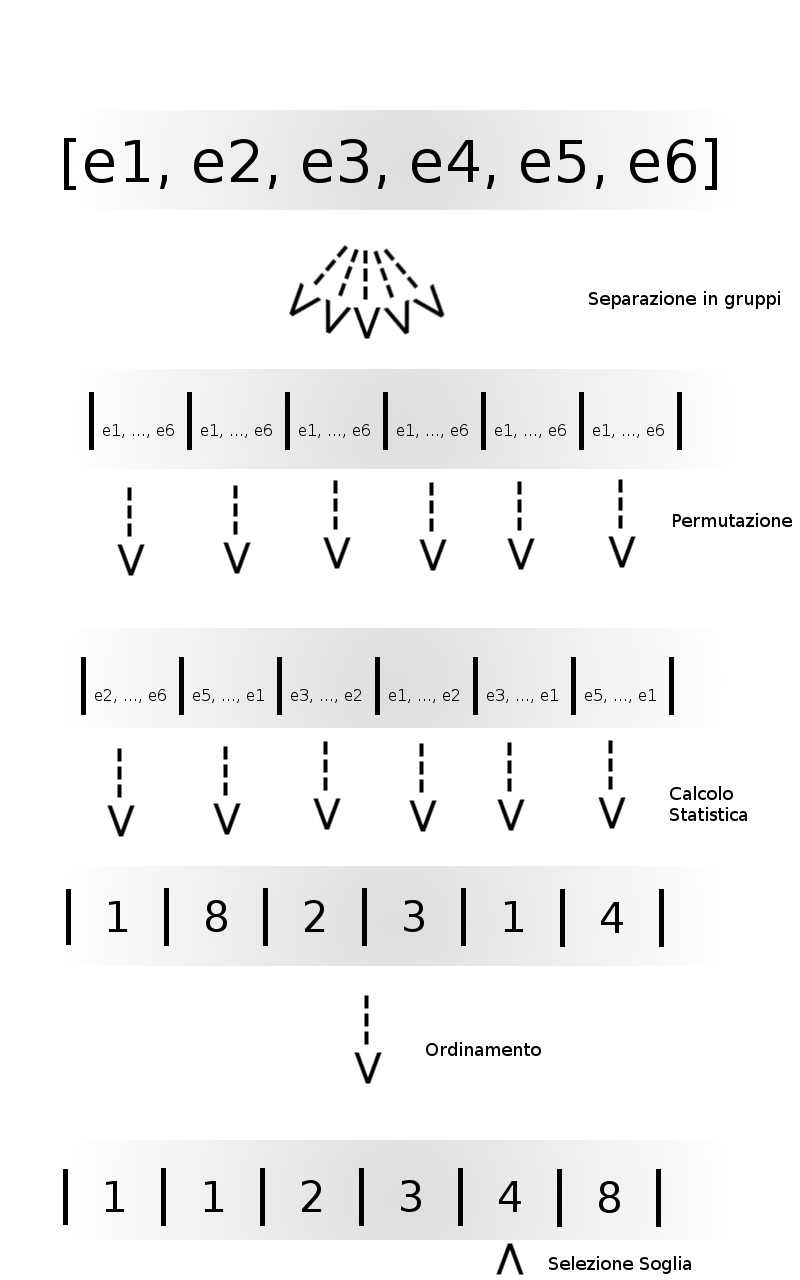
\includegraphics[width=0.7\linewidth]{processo}
\captionof{figure}{Schema riassuntivo Permutation Test}
\end{center}



\subparagraph{Procedura}
Riassumendo, dati un numero di permutationi N e una soglia $\alpha$ la sequenza di operazioni necessarie per operare un test di ipotesi basato sul permutatin test è la seguente.
\begin{enumerate}
	\item Copiare i dati originali
	\item Permutare casualmente i dati originali.
	\item Calcolare la statistica e salvare il risultato.
	\item Se il numeri di risultato raccolti è inferiore a N tornare al punto 1.
	\item Ordinare i risultati.
	\item Confrontare la statistica della popolazione originale contro l'elemento (1-$\alpha$) * dimensione campione. Se la statistica è maggiore, allora sia accetta l'ipotesi nulla, altrimenti la si rifiuta.
\end{enumerate}

